\part{The Foundations of the Mimetic Finite Difference Operators 1D}

\chapter{Introduction and Objectives}

MOLE is an open-source library that implements high-order mimetic
operators~\cite{Corbino2024}.

\section{Staggered grid}

\begin{figure}[ht!]
	\centering
	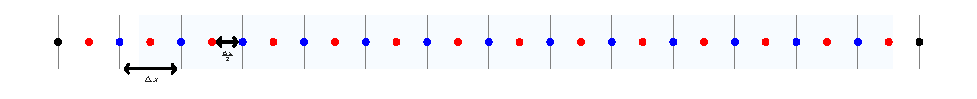
\includegraphics[width=0.8\paperwidth]{staggered}
	\caption{Staggered grid.}
\end{figure}

\begin{equation*}
	Gf_{d}=\vec{0}.
\end{equation*}

\begin{equation*}
	D\vec{v}_{d}=0.
\end{equation*}

Let $U=\left[a,b\right]$.

\begin{equation*}
	\int_{U}
	\vec{v}\cdot\nabla f\dl U+
	\int_{U}
	f\nabla\cdot\vec{v}\dl U=
	\int_{\partial U}
	f\vec{v}\cdot\vec{n}\dl S.
\end{equation*}

\begin{equation*}
	L^{\left(k\right)}=
	D^{\left(k\right)}
	G^{\left(k\right)}.
\end{equation*}

\begin{equation*}
	h
	{\left\langle GF,V\right\rangle}_{P}+
	h
		{\left\langle DV,F\right\rangle}_{Q}=
	F_{N+1}V_{N}-F_{0}V_{0}=
	V^{T}BF.
\end{equation*}

\begin{equation*}
	D^{\left(2\right)}=
	\frac{1}{h}
	\begin{bNiceMatrix}
		1 & 0 & 0 \\
		0 & 1 & 0 \\
		0 & 0 & 1
	\end{bNiceMatrix}.
\end{equation*}

\begin{equation*}
	A=
	\begin{bNiceMatrix}
		a_{11} & \cdots & a_{1c} \\
		\vdots & \ddots & \vdots \\
		a_{r1} & \cdots & a_{rc}
	\end{bNiceMatrix},
	B=
	\begin{bNiceMatrix}
		b_{11} & \cdots & b_{1q} \\
		\vdots & \ddots & \vdots \\
		b_{p1} & \cdots & a_{pq}
	\end{bNiceMatrix}
	A\otimes B\coloneqq
	\begin{bNiceMatrix}
		a_{11}B & \cdots & a_{1c}B \\
		\vdots  & \ddots & \vdots  \\
		a_{r1}B & \cdots & a_{rc}B
	\end{bNiceMatrix}.
\end{equation*}

\begin{equation*}
	D^{\left(k\right)}_{xy}=
	\begin{bNiceMatrix}
		\widehat{I}_{n}\otimes D^{\left(k\right)}_{x} &
		D^{\left(k\right)}_{y}\otimes \widehat{I}_{m}
	\end{bNiceMatrix}.
\end{equation*}

\begin{equation*}
	D^{\left(k\right)}_{xyz}=
	\begin{bNiceMatrix}
		\widehat{I}_{o}\otimes \widehat{I}_{n}\otimes D^{\left(k\right)}_{x}  &
		\widehat{I}_{o} \otimes D^{\left(k\right)}_{y}\otimes \widehat{I}_{m} &
		D^{\left(k\right)}_{z}\otimes \widehat{I}_{n}\otimes \widehat{I}_{m}  &
	\end{bNiceMatrix}.
\end{equation*}

\begin{equation*}
	G^{\left(k\right)}_{xy}=
	\begin{bNiceMatrix}
		\widehat{I}^{T}_{n}\otimes G^{\left(k\right)}_{x} \\
		G^{\left(k\right)}_{y}\otimes \widehat{I}^{T}_{m}
	\end{bNiceMatrix}.
\end{equation*}

\begin{equation*}
	G^{\left(k\right)}_{xyz}=
	\begin{bNiceMatrix}
		\widehat{I}^{T}_{o}\otimes \widehat{I}^{T}_{n}\otimes G^{\left(k\right)}_{x} \\
		\widehat{I}^{T}_{o}\otimes G^{\left(k\right)}_{y}\otimes \widehat{I}^{T}_{m} \\
		G^{\left(k\right)}_{z}\otimes \widehat{I}^{T}_{n}\otimes\widehat{I}^{T}_{m}
	\end{bNiceMatrix}.
\end{equation*}

\chapter{Mimetic Operadors List}

\section{Divergence}

\section{Gradient}

\section{Interpolation from center to nodes}

\section{Interpolation from nodes to center}

\section{Laplacian}

\chapter{Numerical Methods for ODEs}

\todo{Only the methods used in the tutorials: Verlett, RK4, Explicit Euler}

Consider the Initial Value Problem

\begin{equation*}
	\begin{cases}
		\diff{y}{t}=
		f\left(t,y\right), & t\in\left[0,T\right]. \\
		y\left(0\right)=
		y_{0}.             &
	\end{cases}
\end{equation*}

\section{Backward Euler Method}
% https://www.youtube.com/watch?v=HeVsOss1w78
\begin{equation*}
	f\left(t_{n+1},y_{n+1}\right)
	=\diff{y}{t}\approx
	\frac{y_{n+1}-y_{n}}{\Delta t}\implies
	y_{n+1}=
	y_{n}+
	f\left(t_{n+1},y_{n+1}\right)
	\Delta t.
\end{equation*}

The local truncation error is
\begin{math}
	\mathcal{O}
	\left(\Delta t^{2}\right)
\end{math}.
The Butcher table is
\begin{math}
	\renewcommand\arraystretch{1.2}
	\begin{array}
		{c|c}
		1 & 1 \\
		\hline
		  & 1
	\end{array}
\end{math}.

\begin{equation*}
	\begin{cases}
		\diff{y}{t}=
		y\sin t^{2},       & t\in\left[0,5\right]. \\
		y\left(0\right)=2. &
	\end{cases}
\end{equation*}

\begin{equation*}
	S\left(x\right)\coloneqq
	\int_{0}^{x}\sin\left(t^{2}\right)\dl t=
	\sum_{n=0}^{\infty}
	\frac{{\left(-1\right)}^{n}x^{4n+3}}{\left(2n+1\right)!\left(4n+3\right)}.
\end{equation*}

Integramos y obtenemos la solución general.
\begin{align*}
	\iint
	\diff[2]{u}{x}
	\dl x
	\dl x           & =
	\iint
	e^{x}
	\dl x
	\dl x.              \\
	\int
	\diff{u}{x}
	\dl x           & =
	\int
	\left(e^{x}+C_{1}\right)
	\dl x.              \\
	u\left(x\right) & =
	e^{x}+C_{1}x+C_{2}.
\end{align*}
Ahora, apliquemos las condiciones de frontera Robin.
\begin{equation}\label{eq:linearsystem}
	\left\{
	\begin{aligned}
		0
		 & =
		u\left(0\right)-
		\diff{u}{x}[x=0]=
		e^{0}+C_{1}\left(0\right)+C_{2}-
		\left(e^{0}+C_{1}\right)=
		C_{2}-C_{1}. \\
		2e
		 & =
		u\left(1\right)+
		\diff{u}{x}[x=1]=
		e^{1}+C_{1}\left(1\right)+C_{2}+
		\left(e^{1}+C_{1}\right)=
		2e+2C_{1}+C_{2}.
	\end{aligned}
	\right.
\end{equation}
El sistema~\eqref{eq:linearsystem} tiene como solución
$C_{1}=C_{2}=0$.
$\therefore$ la solución
de~\eqref{eq:poisson1drobindconditions} es
$u\left(x\right)=e^{x}$.

\begin{listing}[ht!]
	\tiny
	\centering
	\pathinputminted[frame=single,framesep=10pt,linenos,firstline=1,lastline=13,highlightlines={12}]{octave}{backward_euler.m}
	\caption{Program~\texttt{backward\_euler.m}}
	\label{code:backward_euler.m}
\end{listing}

\begin{figure}[ht!]
	\centering
	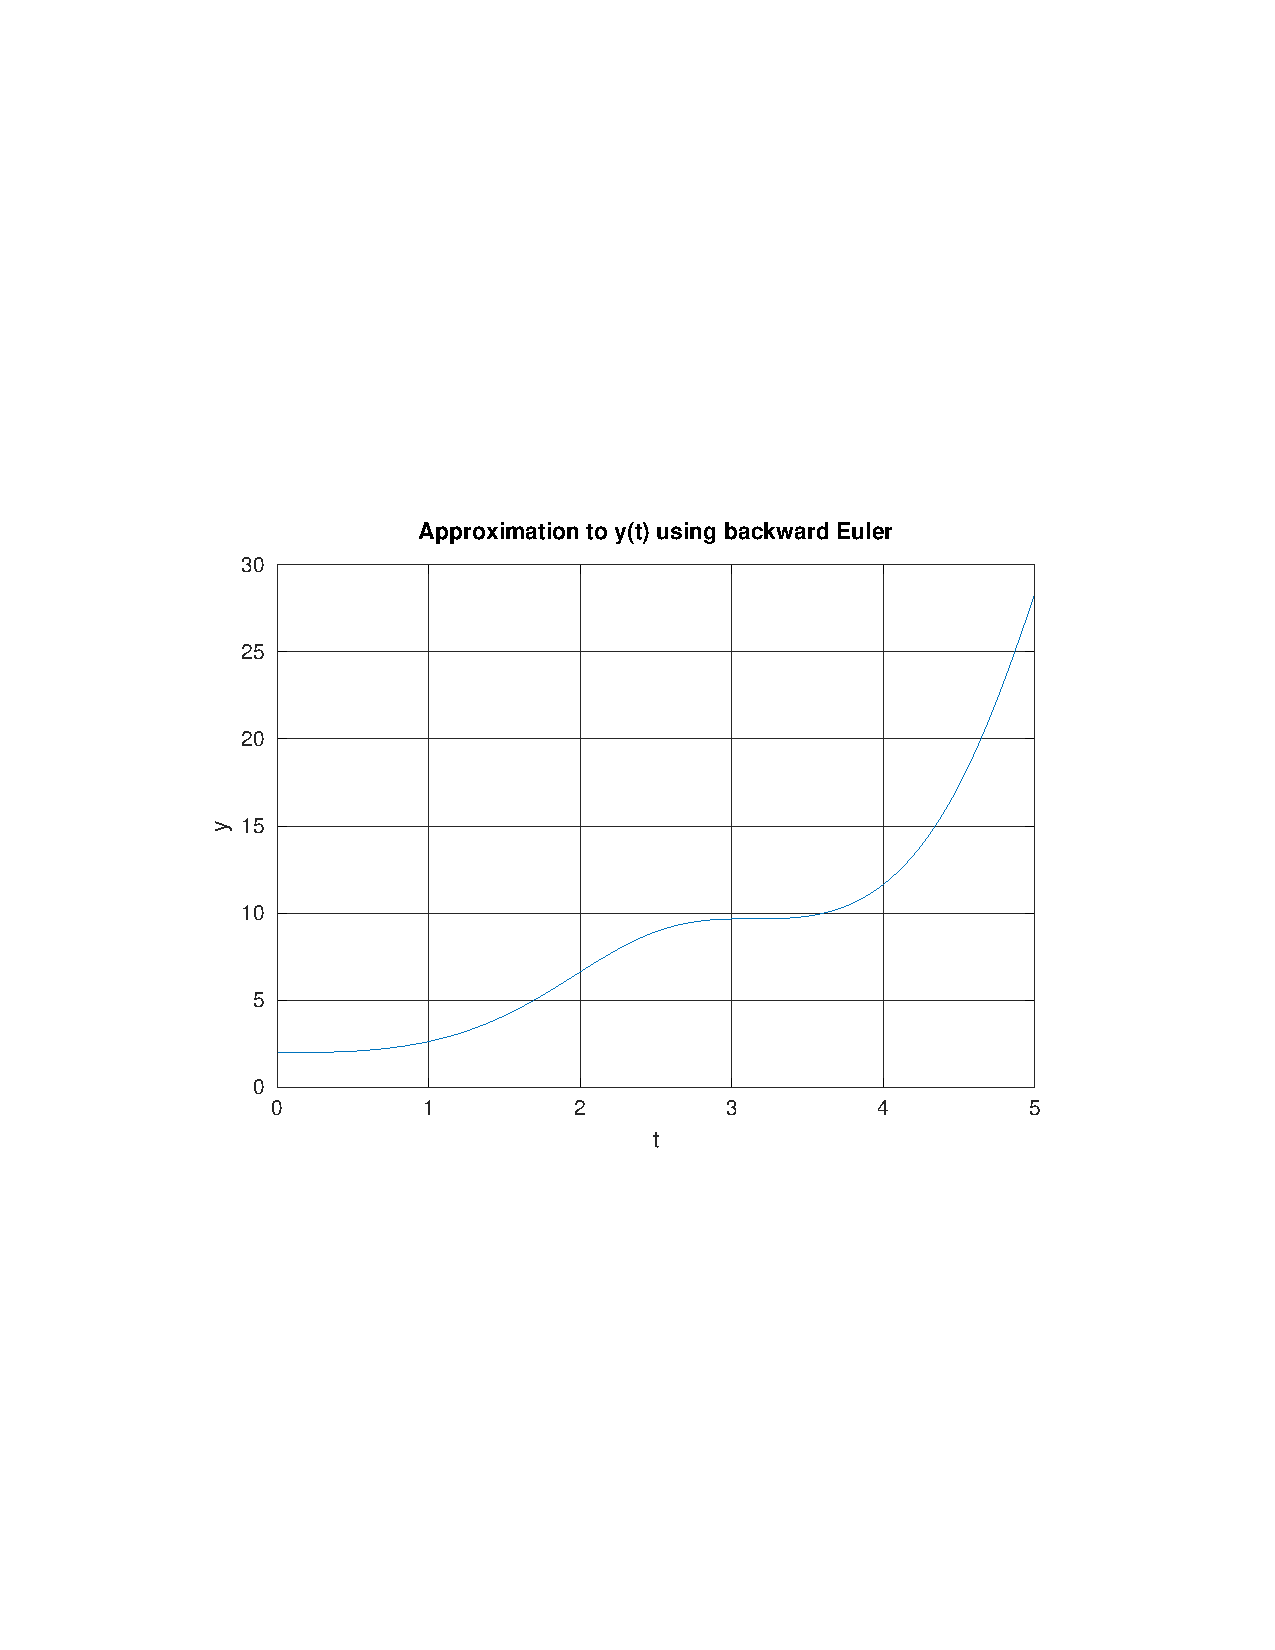
\includegraphics[width=0.55\paperwidth]{backward_euler.pdf}
	\caption{Numerical solution by the Backward Euler Method.}
\end{figure}

\begin{itemize}
	\item

	      \url{https://docs.octave.org/v9.4.0/Ranges.html}

	\item

	      \url{https://docs.octave.org/v9.4.0/Solvers.html#XREFfzero}

	\item

	      \url{https://docs.octave.org/v9.4.0/Object-Sizes.html#XREFsize}

	\item

	      \url{https://docs.octave.org/v9.4.0/Object-Sizes.html#XREFlength}

	\item

	      \url{https://docs.octave.org/v9.4.0/Trigonometry.html#XREFsin}

	\item

	      \url{https://docs.octave.org/v9.4.0/Special-Utility-Matrices.html#XREFzeros}
\end{itemize}

% \url{https://docs.octave.org/v9.4.0/Basic-Vectorization.html}
% \url{https://docs.octave.org/v9.4.0/Ordinary-Differential-Equations.html}

\section{Explicit Runge-Kutta 2}
% https://www.youtube.com/watch?v=HeVsOss1w78
\begin{align*}
	\widetilde{y}_{n+1} & =
	y_{n}+
	f\left(t_{n},y_{n}\right)\Delta t. \\
	y_{n+1}             & =
	y_{n}+
	\frac{\Delta t}{2}
	\left(
	f\left(t_{n},y_{n}\right)+
	f\left(\widetilde{y}_{n+1},t_{n+1}\right)
	\right).
\end{align*}

The local truncation error is
\begin{math}
	\mathcal{O}
	\left(\Delta t^{2}\right)
\end{math}.
The Butcher table is
\begin{math}
	\renewcommand\arraystretch{1.2}
	\begin{array}
		{c|cc}
		0 &             &             \\
		1 & 1           &             \\
		\hline
		  & \frac{1}{2} & \frac{1}{2}
	\end{array}
\end{math}.

\begin{listing}[ht!]
	\tiny
	\centering
	\pathinputminted[frame=single,framesep=10pt,linenos,firstline=1,lastline=14,highlightlines={11-13}]{octave}{RK2.m}
	\caption{Program~\texttt{RK2.m}}
	\label{code:RK2.m}
\end{listing}

\begin{listing}[ht!]
	\tiny
	\centering
	\pathinputminted[frame=single,framesep=10pt,linenos,firstline=1,lastline=14,highlightlines={11-13}]{cpp}{RK2.cpp}
	\caption{Program~\texttt{RK2.m}}
	\label{code:RK2.m}
\end{listing}

\begin{figure}[ht!]
	\centering
	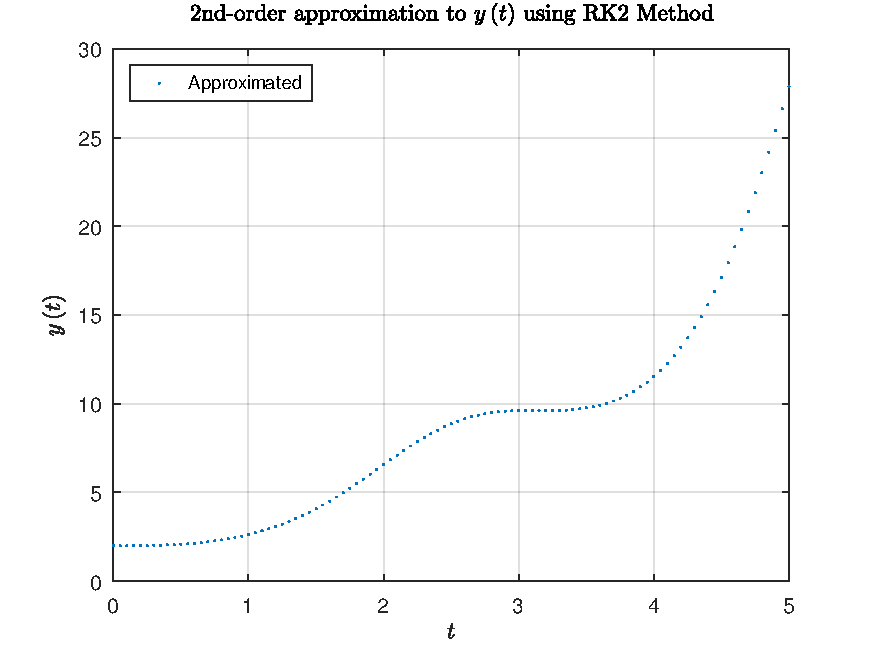
\includegraphics[width=0.55\paperwidth]{RK2.pdf}
	\caption{Numerical solution by the Runge-Kutta 2 Method.}
\end{figure}

\section{Explicit Runge-Kutta 4}
% https://jonshiach.github.io/ODEs-book/_pages/2.3_RK4_Derivation.html
% https://www.youtube.com/watch?v=qUe_kR7QoBU

\begin{align*}
	k_{1}   & =
	f\left(t_{n},y_{n}\right).                                            \\
	k_{2}   & =
	f\left(t_{n}+\frac{\Delta t}{2},y_{n}+\Delta t\frac{k_{1}}{2}\right). \\
	k_{3}   & =
	f\left(t_{n}+\frac{\Delta t}{2},y_{n}+\frac{\Delta k_{2}}{2}\right).  \\
	k_{4}   & =
	f\left(t_{n}+\Delta t,y_{n}+\Delta t k_{3}\right).                    \\
	y_{n+1} & =
	y_{n}+
	\frac{1}{6}\left(k_{1}+2k_{2}+2k_{3}+k_{4}\right).
\end{align*}

The local truncation error is
\begin{math}
	\mathcal{O}
	\left(\Delta t^{4}\right)
\end{math}.
The Butcher table is
\begin{math}
	\renewcommand\arraystretch{1.2}
	\begin{array}
		{c|cccc}
		0           &             &             &             &             \\
		\frac{1}{2} & \frac{1}{2} &             &             &             \\
		\frac{1}{2} & 0           & \frac{1}{2} &             &             \\
		1           & 0           & 0           & 1           &             \\
		\hline
		            & \frac{1}{6} & \frac{4}{6} & \frac{4}{6} & \frac{1}{6}
	\end{array}
\end{math}.

\begin{listing}[ht!]
	\tiny
	\centering
	\pathinputminted[frame=single,framesep=10pt,linenos,firstline=1,lastline=16,highlightlines={11-15}]{octave}{RK4.m}
	\caption{Program~\texttt{RK4.m}}
	\label{code:RK2.m}
\end{listing}

\begin{figure}[ht!]
	\centering
	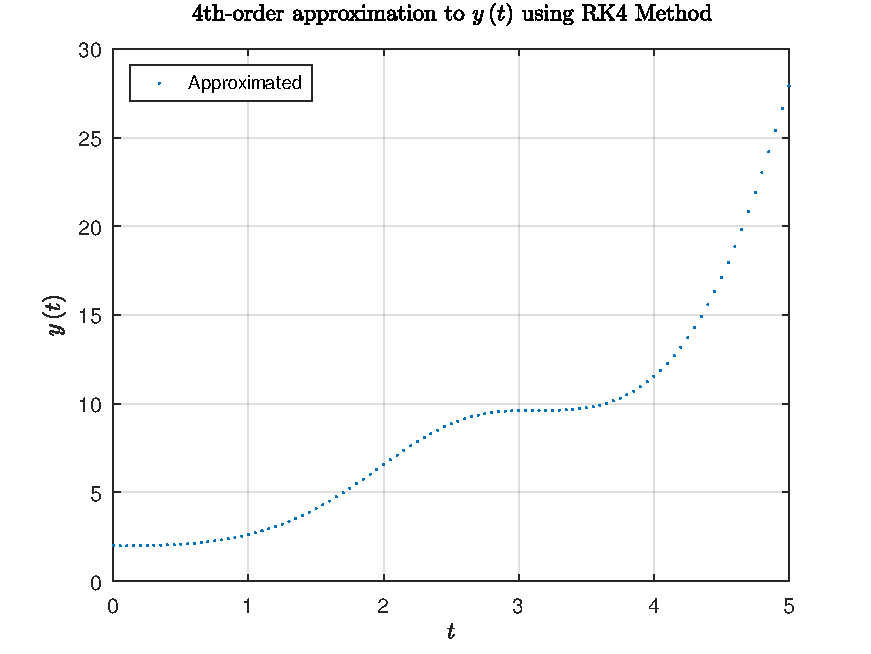
\includegraphics[width=0.55\paperwidth]{RK4.pdf}
	\caption{Numerical solution by the Runge-Kutta 4 Method.}
\end{figure}

\section{Verlett}

\chapter{Numerical Solutions of Boundary Value Problems}

\chapter{Numerical Methods for PDEs}

\section{von Neumann Stability Criterion}

\section{Stability and Convergence Analysis}

\section{Method of characteristics}

\cite{Choksi2022,Arrigo2023}

Let's consider the problem of

\begin{equation*}
	\begin{cases}
		\difcp{u}{t}+
		c\difcp{u}{x}=0,   & x\in\left(0,1\right),\, t>0. \\
		u\left(0,t\right)=
		u\left(1,t\right), & t>0.                         \\
		u\left(x,0\right)=
		g\left(x\right),   & x\in\left[0,1\right].
	\end{cases}
\end{equation*}

Consider the problem for the explicit form of linear first-oder
PDEs in two independent variables

\begin{equation*}
	\begin{cases}
		a
		\left(x,y\right)
		\difcp{u}{x}+
		b
		\left(x,y\right)
		\difcp{u}{y}=
		c_{1}
		\left(x,y\right)
		u+
		c_{2}
		\left(x,y\right), \\
		u\left(x,y\right)
		\text{given for}
		\left(x,y\right)\in
		\Gamma.
	\end{cases}
\end{equation*}

to be solved in some domain
\begin{math}
	\Omega\subset
	\mathbb{R}^{2}
\end{math}
with data given on some curve
\begin{math}
	\Gamma\subset
	\overline\Omega
\end{math}.

Often the
\begin{math}
	\Gamma\subset
	\partial\Omega\subset
	\mathbb{R}^{2}
\end{math}
it will just be one of the coordinate axes.

We find the characteristics, i.e., the curves which follow these
directions, by solving

\begin{equation*}
	\diff{x}{s}=
	a
	\left(
	x\left(s\right),
	y\left(s\right)
	\right),\qquad
	\diff{y}{s}=
	b
	\left(
	x\left(s\right),
	y\left(s\right)
	\right).
\end{equation*}

Now suppose $u$ is a solution to the PDE.
Let $z\left(s\right)$ denote the values of the solution $u$ along a
characteristic; i.e.,

\begin{equation*}
	z
	\left(s\right)\coloneqq
	u
	\left(
	x\left(s\right),
	y\left(s\right)
	\right).
\end{equation*}

Then by the chain rule, we have
\begin{align*}
	\diff{z}{s}
	 & =
	\difcp{u}{x}
	\left(
	x\left(s\right),
	y\left(s\right)
	\right)
	\diff{x}{s}
	\left(
	x\left(s\right),
	y\left(s\right)
	\right)+
	\difcp{u}{y}
	\left(
	x\left(s\right),
	y\left(s\right)
	\right)
	\diff{y}{s}
	\left(
	x\left(s\right),
	y\left(s\right)
	\right). \\
	\diff{z}{s}
	 & =
	\difcp{u}{x}
	\left(
	x\left(s\right),
	y\left(s\right)
	\right)
	a
	\left(
	x\left(s\right),
	y\left(s\right)
	\right)+
	\difcp{u}{y}
	\left(
	x\left(s\right),
	y\left(s\right)
	\right)
	b
	\left(
	x\left(s\right),
	y\left(s\right)
	\right). \\
	\diff{z}{s}
	 & =
	c_{1}
	\left(
	x\left(s\right),
	y\left(s\right)
	\right)
	z
	\left(s\right)+
	c_{2}
	\left(
	x\left(s\right),
	y\left(s\right)
	\right).
\end{align*}

\begin{definition}{Characteristics equations}{characteristics}
	There are three \emph{dependent variables} $x$, $y$ and $z$ and
	one \emph{independent} variable $s$.
	\begin{equation*}
		\begin{cases}
			\diff{x}{s}
			\left(s\right) & =
			a
			\left(
			x\left(s\right),
			y\left(s\right)
			\right).           \\
			\diff{y}{s}
			\left(s\right) & =
			b
			\left(
			x\left(s\right),
			y\left(s\right)
			\right).           \\
			\diff{z}{s}
			\left(s\right) & =
			c_{1}
			\left(
			x\left(s\right),
			y\left(s\right)
			\right)
			z
			\left(s\right)+
			c_{2}
			\left(
			x\left(s\right),
			y\left(s\right)
			\right).
		\end{cases}
	\end{equation*}
\end{definition}

\begin{figure}[ht!]
	\centering
	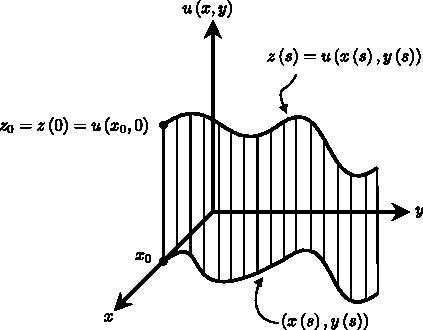
\includegraphics[width=0.35\paperwidth]{characteristics}
	\caption{The solution $u$ is described by the surface defined by
		$z=u\left(x,y\right)$.
		From any point $x_{0}$ on the $x$-axis, there is a curve
		$\left(x\left(s\right),y\left(s\right)\right)$ in the
		$xy$-plane, upon which wa can calculate the solution
		$z=u\left(x\left(s\right),y\left(s\right)\right)$.
		Knowing only the structure of the PDE, $x_{0}$ and $z_{0}$ we
		can solve ODEs to find the part of the solution surface which
		lies above the curve.}
\end{figure}

\begin{equation*}
	a\left(x,y\right)\diffp{u}{x}+
	b\left(x,y\right)\diffp{u}{y}=
	c_{1}\left(x,y\right)u+
	c_{2}\left(x,y\right),
	u\text{ given for }\left(x,y\right)\in\Gamma
\end{equation*}
where we have a linear PDE in the independent variables $x$ and $y$
with a given functions $a$, $b$, $c_{1}$ and $c_{2}$ of $\left(x,y\right)$.
$\Gamma\subset\partial\Omega$.
We find the characteristics, i.e., the curves which follow these directions, by solving
\begin{align*}
	\diff{x}{s}     & =
	a\left(x\left(s\right),y\left(s\right)\right). \\
	\diff{y}{s}     & =
	b\left(x\left(s\right),y\left(s\right)\right). \\
	z\left(s\right) & =
	u\left(x\left(s\right),y\left(s\right)\right).
\end{align*}

\begin{equation*}
	\diff{z}{s}=
	c_{1}\left(x\left(s\right),y\left(s\right)\right)
	z\left(s\right)+
	c_{2}\left(x\left(s\right),y\left(s\right)\right).
\end{equation*}

\section{Method of separation of variables}

% https://sci-hub.se/10.1137/S0895479801398025
% https://github.com/nutrik/pymole?tab=readme-ov-file

\section{Getting started with MOLE}
\subsection{Compiling and running the first code}

\section{Test $1$}

\begin{listing}[ht!]
	\tiny
	\centering
	\pathinputminted[frame=single,framesep=10pt,linenos,firstline=1,lastline=33,highlightlines={9-19}]{cpp}{test1.cpp}
	\caption{Program~\texttt{test1.cpp}}
	\label{code:test1.cpp}
\end{listing}

\begin{listing}[ht!]
	\tiny
	\centering
	\pathinputminted[frame=single,framesep=10pt,linenos,firstline=1,lastline=21,highlightlines={8-19}]{octave}{test1.m}
	\caption{Program~\texttt{test1.m}}
	\label{code:test1.m}
\end{listing}

\section{Test $2$}

\begin{listing}[ht!]
	\tiny
	\centering
	\pathinputminted[frame=single,framesep=10pt,linenos,firstline=1,lastline=28,highlightlines={9-20}]{cpp}{test2.cpp}
	\caption{Program~\texttt{test2.cpp}}
	\label{code:test2.cpp}
\end{listing}

\begin{listing}[ht!]
	\tiny
	\centering
	\pathinputminted[frame=single,framesep=10pt,linenos,firstline=1,lastline=21,highlightlines={8-19}]{octave}{test2.m}
	\caption{Program~\texttt{test2.m}}
	\label{code:test2.m}
\end{listing}

\section{Test $3$}

\begin{listing}[ht!]
	\tiny
	\centering
	\pathinputminted[frame=single,framesep=10pt,linenos,firstline=1,lastline=27,highlightlines={8-19}]{cpp}{test3.cpp}
	\caption{Program~\texttt{test3.cpp}}
	\label{code:test3.cpp}
\end{listing}

\begin{listing}[ht!]
	\tiny
	\centering
	\pathinputminted[frame=single,framesep=10pt,linenos,firstline=1,lastline=21,highlightlines={8-19}]{octave}{test3.m}
	\caption{Program~\texttt{test3.m}}
	\label{code:test3.m}
\end{listing}

\section{Test $4$}

\begin{listing}[ht!]
	\tiny
	\centering
	\pathinputminted[frame=single,framesep=10pt,linenos,firstline=1,lastline=39,highlightlines={10-39}]{cpp}{test4.cpp}
	\caption{Program~\texttt{test4.cpp}}
	\label{code:test4.cpp}
\end{listing}

\begin{listing}[ht!]
	\tiny
	\centering
	\pathinputminted[frame=single,framesep=10pt,linenos,firstline=1,lastline=48,highlightlines={15-44}]{octave}{test4.m}
	\caption{Program~\texttt{test4.m}}
	\label{code:test4.m}
\end{listing}

\section{Test $5$}

\begin{listing}[ht!]
	\tiny
	\centering
	\pathinputminted[frame=single,framesep=10pt,linenos,firstline=1,lastline=61,highlightlines={9-53}]{cpp}{test5.cpp}
	\caption{Program~\texttt{test5.cpp}}
	\label{code:test5.cpp}
\end{listing}

\begin{listing}[ht!]
	\tiny
	\centering
	\pathinputminted[frame=single,framesep=10pt,linenos,firstline=1,lastline=55,highlightlines={10-53}]{octave}{test5.m}
	\caption{Program~\texttt{test5.m}}
	\label{code:test5.m}
\end{listing}
